% Provenance (never printed): see sources/outline_sources.md (Year 1:
% observational astronomy, photometry). Telescopes, angular resolution,
% gratings, the Doppler effect and the black-body laws are owned by the
% physics series and recalled here. Curves computed in
% figdata/bachelor-1/{blackbody_bands, extinction_line}.py; numbers of the
% exercises and problem in the Book 3 scratch calculator ch02.py.
\chapter{Telescopios, detectores y fotometría}\label{ch:b1:observing-the-sky}

Todo lo que la astronomía sabe de las estrellas, aparte de unos pocos meteoritos y
de las muestras traídas de la Luna y de los asteroides, lo ha aprendido de la luz
que envían. Esa luz atraviesa la atmósfera terrestre, que absorbe franjas enteras de
longitudes de onda y emborrona el resto; la recoge un espejo cuyo tamaño limita
tanto lo débil como lo fino que puede ser el detalle; la cuenta un detector que
convierte fotones en electrones, y cada cuenta lleva una incertidumbre estadística.
Antes de que un brillo se convierta en una \omterm{def:b1:observing-the-sky:flux}{luminosidad} o en una distancia, hay que
entender y corregir cada uno de estos pasos. Este capítulo sigue la luz desde la
estrella hasta el número: las ventanas de la atmósfera y la ley de la extinción, el
telescopio y el \omterm{def:b1:observing-the-sky:seeing}{seeing}, el detector y su ruido, y después las magnitudes, los
paralajes y los colores que convierten los \omterm{def:b1:observing-the-sky:flux}{flujos} medidos en propiedades de las
estrellas. La misma atmósfera, vista desde abajo, es el tema de los capítulos sobre
el clima (\cref{ch:b1:radiation-heat-transport}); la misma fotometría, aplicada a los
planetas, abre el capítulo siguiente (\cref{ch:b1:comparative-planetology}).

\begin{recall}
Un objetivo de telescopio recoge la luz a lo largo de su abertura y forma una imagen
en su foco; la difracción por una abertura de diámetro $D$ limita el ángulo más
pequeño que puede separar a unos $1.22\,\lambda/D$, el criterio de Rayleigh (el
volumen de primer año de los libros de física). Una red dispersa la luz según su
longitud de onda (segundo año), y una fuente que se mueve a lo largo de la visual
desplaza sus líneas espectrales por efecto Doppler (año 12). Un cuerpo en equilibrio
térmico emite el espectro del cuerpo negro, cuyo máximo obedece a la ley de Wien
(segundo año). En química, la absorbancia de una disolución crece en proporción a la
longitud del camino recorrido.
\end{recall}

\section{Las ventanas de la atmósfera}

La atmósfera es transparente a unas longitudes de onda y opaca a otras. La radiación
la absorben sobre todo el vapor de agua, el dióxido de carbono y el ozono, y, en las
longitudes de onda más cortas, los átomos y moléculas de la alta atmósfera.
% ledger: nasa:ems-absorbers

\begin{definition}[Ventana atmosférica]\label{def:b1:observing-the-sky:window}
Una \emph{ventana atmosférica}\index{ventana atmosférica} es una franja de longitudes
de onda en la que la atmósfera deja pasar la mayor parte de la radiación que llega a
su parte superior hasta el suelo. La \emph{ventana óptica} se
extiende desde el ultravioleta cercano hasta el infrarrojo cercano; la
\emph{ventana de radio} va desde longitudes de onda de un
centímetro aproximadamente hasta unos diez metros.
\end{definition}

La figura siguiente esboza la opacidad de la atmósfera desde los rayos gamma hasta las
ondas de radio largas. Los rayos gamma, los rayos X y el ultravioleta por debajo de
unos \qty{0.3}{\micro\metre} nunca llegan al suelo: se observan desde el espacio. La
luz visible pasa, con cierto emborronamiento. La mayor parte del infrarrojo lo absorben
el vapor de agua y el dióxido de carbono, salvo en unas estrechas ventanas que
aprovechan los observatorios terrestres de sitios altos y secos; las \omterm{def:b1:observing-the-sky:magnitude}{bandas
fotométricas} del infrarrojo cercano se sitúan en ellas, en \qty{1.24}{\micro\metre},
\qty{1.65}{\micro\metre} y \qty{2.16}{\micro\metre}. Las longitudes de onda desde unas
\qty{30}{\micro\metre} hasta un milímetro vuelven a quedar bloqueadas; las ondas de
radio de unos pocos centímetros hasta unos diez metros pasan, incluso a través de las
nubes; las más largas las refleja la ionosfera.
% ledger: nasa:opacity-windows, baldry:2mass-pivot

\begin{omfigure}
\begin{tikzpicture}[x=1.0cm, y=2.2cm, font=\scriptsize]
% x = log10(lambda / 1 m) + 10 ; opacity 0..1 (schematic, after the NASA figure)
\fill[omSea!20] (0,0) rectangle (13,1.05);
\fill[brown!50] (0,0) -- (0,1) -- (3.45,1) -- (3.52,0.05) -- (4.03,0.05)
  -- (4.06,0.6) -- (4.09,0.15) -- (4.15,0.6) -- (4.22,0.15) -- (4.28,0.6)
  -- (4.34,0.15) -- (4.42,0.7) -- (4.55,0.25) -- (4.65,0.8) -- (4.9,0.2)
  -- (5.12,0.2) -- (5.25,0.7) -- (5.4,1) -- (7.0,1) -- (7.3,0.6) -- (7.6,0.75)
  -- (8.0,0.5) -- (8.5,0.03) -- (11.0,0.03) -- (11.3,1) -- (13,1) -- (13,0)
  -- cycle;
\draw[black!70] (0,0) rectangle (13,1.05);
\foreach \x in {0,...,13} { \draw (\x,0) -- (\x,-0.05); }
\foreach \x/\l in {0/0.1 nm, 2/10 nm, 4/1 \unit{\micro m}, 6/100 \unit{\micro m}, 8/1 cm,
  10/1 m, 12/100 m}
  { \node[below] at (\x,-0.05) {\l}; }
\foreach \y/\l in {0/0, 0.5/50, 1/100}
  { \draw (0,\y) -- (-0.1,\y); \node[left] at (-0.1,\y) {\l}; }
\node[rotate=90] at (-0.75,0.5) {opacidad (\%)};
\node at (6.5,-0.42) {\small longitud de onda (escala logarítmica)};
\node[align=center] at (1.7,0.75) {rayos gamma, rayos X,\\ ultravioleta};
\node[align=center] at (6.2,0.75) {infrarrojo\\ lejano};
\node[align=center] at (9.75,0.5) {ventana de radio};
\node[omThm] at (4.15,0.86) {J H K};
\draw[-{Stealth}] (2.6,1.25) node[above] {ventana óptica} -- (3.75,1.07);
\draw[-{Stealth}] (5.9,1.25) node[above] {ventanas infrarrojas} -- (4.6,1.07);
\end{tikzpicture}

{\small La opacidad de la atmósfera a la radiación que llega desde el espacio, desde
\qty{0.1}{nm} hasta \qty{1}{km} (escala logarítmica). Esquema, a partir de una figura
de la NASA de dominio público: aquí solo importan las ventanas, no la forma exacta de
cada banda de absorción. J, H y K marcan las \omterm{def:b1:observing-the-sky:magnitude}{bandas fotométricas} del infrarrojo
cercano.}
% ledger: nasa:opacity-windows, nasa:ems-absorbers, baldry:2mass-pivot
\end{omfigure}

\subsection*{Extinción}

Incluso dentro de la ventana óptica la atmósfera quita parte de la luz, por absorción
y por dispersión sobre moléculas y aerosoles. Una capa delgada de espesor $\mathrm ds$
a lo largo del rayo retira una fracción de la intensidad proporcional a $\mathrm ds$:
$\mathrm dI = -\kappa I\,\mathrm ds$, donde el coeficiente de extinción $\kappa$
(por metro) depende de la longitud de onda y de la composición del aire a esa altura.
Es la ley de la absorbancia de una disolución, aplicada a una columna de aire.

\begin{proposition}[Ley de Bouguer]\label{prop:b1:observing-the-sky:bouguer}
A lo largo de un rayo que atraviesa un medio absorbente, la intensidad disminuye así:
\[
  I = I_0\,e^{-\tau}, \qquad \tau = \int_0^s \kappa\,\mathrm ds' ,
\]
donde $I_0$ es la intensidad que entra en el medio y $\tau$, la profundidad óptica del
camino, es un número puro.
En una atmósfera plano-paralela, una estrella a la distancia cenital $z$ (el ángulo
entre su dirección y la vertical) se observa a través de la profundidad óptica
$\tau(z) = \tau_0\sec z$, donde $\tau_0$ es la profundidad óptica en el \omterm{def:b1:spherical-astronomy:celestial-sphere}{cenit}.
\end{proposition}

\begin{proof}
La ecuación $\mathrm dI/I = -\kappa\,\mathrm ds$ se separa: integrando desde la parte
superior de la atmósfera ($I = I_0$, $s = 0$) hasta el observador se obtiene
$\ln(I/I_0) = -\int_0^s\kappa\,\mathrm ds'$. En una atmósfera plano-paralela, $\kappa$
depende solo de la altura $y$, y un rayo inclinado $z$ respecto de la vertical recorre
$\mathrm ds = \mathrm dy/\cos z$ para subir $\mathrm dy$. Por tanto,
$\tau(z) = \int \kappa(y)\,\mathrm dy/\cos z = \tau_0\sec z$.
\end{proof}

\begin{definition}[Masa de aire, coeficiente de extinción atmosférica]\label{def:b1:observing-the-sky:extinction}
La \emph{masa de aire}\index{masa de aire} $X$ de una observación es la profundidad
óptica de la visual dividida por la profundidad óptica en el \omterm{def:b1:spherical-astronomy:celestial-sphere}{cenit}:
$X = \tau(z)/\tau_0$. Vale 1 en el \omterm{def:b1:spherical-astronomy:celestial-sphere}{cenit} y, para una atmósfera plano-paralela,
$X = \sec z$. El \emph{coeficiente de extinción atmosférica}\index{coeficiente de extinción atmosférica}
$k$ en una banda dada es el oscurecimiento, en magnitudes, que produce una masa de aire,
de modo que una estrella de magnitud $m_0$ por encima de la atmósfera se observa en
\[
  m = m_0 + kX .
\]
\end{definition}

Las magnitudes se definen en \cref{sec:b1:observing-the-sky:magnitudes}; basta aquí con
saber que un oscurecimiento por el factor $e^{-\tau}$ añade
$2.5\log_{10}e\;\tau = 1.086\,\tau$ magnitudes, de modo que $k = 1.086\,\tau_0$.
La \omterm{def:b1:observing-the-sky:extinction}{masa de aire} plano-paralela es excelente hasta una altura de unos \ang{30} ($X = 2$)
y falla cerca del horizonte, donde $\sec z$ crece sin límite mientras que el camino real
a través de una atmósfera curva sigue siendo finito; por esa razón, y por el
emborronamiento que crece con el camino, los observadores evitan las alturas bajas.

\begin{method}[La recta de extinción]\label{met:b1:observing-the-sky:extinction-line}
Para hallar la magnitud $m_0$ que tendría una estrella por encima de la atmósfera:
\begin{enumerate}
  \item mídase la magnitud $m$ de la estrella, o de una estrella patrón, a varias \omterm{def:b1:observing-the-sky:extinction}{masas
        de aire} a lo largo de la noche, mientras sube o baja;
  \item calcúlese cada \omterm{def:b1:observing-the-sky:extinction}{masa de aire} a partir de la distancia cenital, $X = \sec z$;
  \item represéntese $m$ frente a $X$ y ajústese una recta por mínimos cuadrados;
  \item la pendiente es el coeficiente de extinción $k$ de la noche en esa banda; la
        ordenada en el origen, en $X = 0$, es $m_0$.
\end{enumerate}
El mismo $k$ corrige después cualquier otra estrella observada esa noche en la misma
banda: $m_0 = m - kX$.
\end{method}

\begin{example}
Una noche se midió seis veces una estrella en la banda V:
\begin{center}
\small
\begin{tabular}{lcccccc}
\hline
$X$ & 1.05 & 1.18 & 1.36 & 1.62 & 1.95 & 2.31 \\
$m$ & 8.024 & 8.031 & 8.072 & 8.104 & 8.171 & 8.216 \\
\hline
\end{tabular}
\end{center}
La recta de mínimos cuadrados, dibujada en la figura siguiente, tiene pendiente
$k = \qty{0.160}{\mag}$ por \omterm{def:b1:observing-the-sky:extinction}{masa de aire} y ordenada en el origen $m_0 = 7.851$. Los
puntos se dispersan alrededor de ella \num{0.006} magnitudes, la precisión de una buena
noche de fotometría. En el \omterm{def:b1:spherical-astronomy:celestial-sphere}{cenit} la estrella se oscurece \num{0.16} magnitudes, una
pérdida de $1 - 10^{-0.4\times0.160} = \qty{14}{\percent}$ de su luz.
\end{example}

\begin{omfigure}
\begin{tikzpicture}
\begin{axis}[omrecord, width=0.62\linewidth, height=5.4cm, xmin=0, xmax=2.5,
  ymin=7.80, ymax=8.28, y dir=reverse, xlabel={masa de aire $X$},
  ylabel={magnitud $m$}, yticklabel style={/pgf/number format/fixed,
  /pgf/number format/precision=2}, tick label style={font=\scriptsize},
  label style={font=\small}]
\addplot[omThm, line width=0.9pt, dashed] table[x=X, y=m] {figdata/out/bachelor-1-extinction_line-fit.dat};
\addplot[only marks, mark=*, mark size=1.6pt, omDef] table[x=X, y=m] {figdata/out/bachelor-1-extinction_line-obs.dat};
\node[font=\scriptsize, right, fill=white, inner sep=1pt] at (axis cs:0.05,7.83) {$m_0 = 7.851$};
\node[font=\scriptsize, fill=white, inner sep=1pt, rotate=-10] at (axis cs:0.95,8.10) {pendiente $k = 0.160$};
\end{axis}
\end{tikzpicture}

{\small Una recta de extinción: la magnitud de una estrella a seis \omterm{def:b1:observing-the-sky:extinction}{masas de aire}
(puntos) y la recta de mínimos cuadrados, prolongada hasta $X = 0$, la magnitud por
encima de la atmósfera. Las magnitudes crecen hacia abajo: una estrella más débil se
sitúa más abajo.}
\end{omfigure}

\subsection*{Seeing}

El aire sobre un telescopio nunca está quieto. Celdas de aire a temperaturas algo
distintas, y por tanto con índices de refracción algo distintos, se desplazan a
través del haz y lo desvían en pequeños ángulos al azar, que cambian muchas veces por
segundo. El ojo ve titilar una estrella; una exposición larga registra una mancha
borrosa mucho mayor que la figura de difracción del telescopio.

\begin{definition}[Seeing]\label{def:b1:observing-the-sky:seeing}
El \emph{seeing}\index{seeing} de un lugar es el diámetro angular de la imagen de una
fuente puntual emborronada por la turbulencia atmosférica en una exposición larga,
medido como la anchura a media altura de la imagen, en segundos de arco.
\end{definition}

El \omterm{def:b1:observing-the-sky:seeing}{seeing} cambia de una noche a otra y de una hora a otra. Los lugares se eligen por
él: en la cima del Mauna Kea, a \qty{4204}{m}, el \omterm{def:b1:observing-the-sky:seeing}{seeing} mediano de la atmósfera libre
es de unos \ang{;;0.40}, de unos \ang{;;0.45} en invierno a \ang{;;0.35} en verano, y la
décima parte de las mejores noches queda por debajo de unos \ang{;;0.25}; el mismo lugar
tiene por encima solo \qty{0.9}{mm} de vapor de agua precipitable mediano, lo que abre
sus ventanas infrarrojas.
% ledger: cfht:site, cfht:seeing

\section{Telescopios y resolución}

Un telescopio hace dos cosas: recoge la luz a lo largo del área de su objetivo y forma
una imagen en la que los detalles quedan separados. El área de recogida crece como
$D^2$: un espejo dos veces más ancho capta cuatro veces más fotones en el mismo tiempo
y alcanza estrellas cuatro veces más débiles. La resolución la limita la difracción, a
unos $1.22\,\lambda/D$, y el \omterm{def:b1:observing-the-sky:seeing}{seeing}.

\begin{example}
El Telescopio Canadá--Francia--Hawái, en el Mauna Kea, tiene una abertura de
\qty{3.58}{m}. A \qty{550}{nm} su límite de difracción es
\[
  1.22\times\frac{\qty{550e-9}{m}}{\qty{3.58}{m}} = \qty{1.87e-7}{rad}
  = \ang{;;0.039},
\]
diez veces más fino que el \omterm{def:b1:observing-the-sky:seeing}{seeing} mediano de \ang{;;0.40} del mismo lugar. Los dos
límites son iguales para un espejo de diámetro $D = 1.22\lambda/\theta =
1.22\times\qty{550e-9}{m}/(\num{0.40}/\num{206265}) = \qty{0.35}{m}$: cualquier
telescopio terrestre más ancho que unos \qty{35}{cm} está limitado por el \omterm{def:b1:observing-the-sky:seeing}{seeing}, y no
por su propia óptica, a longitudes de onda visibles.
% ledger: cfht:aperture, cfht:seeing
\end{example}

Un gran telescopio terrestre gana, por tanto, área de recogida, no nitidez, a menos que
corrija la turbulencia. La \emph{óptica adaptativa} lo hace: un sensor mide, muchas
veces por segundo, cómo se deforma el frente de ondas de una estrella brillante (o de
una estrella artificial creada por un láser en la alta atmósfera), y un espejo delgado,
doblado por muchos actuadores pequeños, cancela la deformación. La corrección funciona
mejor en el infrarrojo, donde la turbulencia es más lenta y más débil, y en un campo
pequeño alrededor de la estrella guía. En el espacio no hay \omterm{def:b1:observing-the-sky:seeing}{seeing} en absoluto.

\section{Detectores}

El ojo integra la luz durante una fracción de segundo y responde a una pequeña fracción
de los fotones que le llegan. Las placas fotográficas integraban durante horas, pero
registraban solo una pequeña fracción de la luz. La astronomía moderna usa detectores de
fotones hechos de semiconductores, en los que cada fotón absorbido con energía
suficiente libera un electrón.

\begin{definition}[Eficiencia cuántica, relación señal-ruido]\label{def:b1:observing-the-sky:detector}
La \emph{eficiencia cuántica}\index{eficiencia cuántica} $\eta$ de un detector a una
longitud de onda dada es la fracción de los fotones incidentes que registra como
fotoelectrones: $\eta = N_\mathrm{e}/N_\gamma$. La \emph{relación señal-ruido}\index{relación señal-ruido}
de una medida es la señal medida dividida por su desviación típica, el tamaño típico de
su error aleatorio.
\end{definition}

El \emph{dispositivo de carga acoplada} (CCD) es el detector estándar de la ventana
óptica. Es una lámina delgada de silicio dividida en una malla de píxeles, cada uno de
ellos un pozo de potencial que almacena los electrones liberados por los fotones que
absorbe durante la exposición. Al final de la exposición, unos voltajes aplicados en
secuencia a los electrodos desplazan las cargas de píxel en píxel, fila a fila, hacia un
único amplificador que las mide una a una; la imagen es la tabla de los recuentos. Un
CCD registra una gran fracción de los fotones incidentes en casi todo el visible, su
respuesta es proporcional a la luz recibida hasta una carga máxima por píxel (su
\emph{pozo lleno}), y puede integrar durante horas. Las matrices
infrarrojas funcionan con el mismo principio, con otros semiconductores, leídas píxel a
píxel.

Los fotones llegan al azar. Si una fuente envía en promedio $N$ fotoelectrones durante
una exposición, el recuento realmente registrado fluctúa de una exposición a la
siguiente con la desviación típica $\sqrt N$ (estadística de Poisson, la del recuento de
sucesos raros e independientes).

\begin{proposition}[Ruido de fotones]\label{prop:b1:observing-the-sky:snr}
Cuando domina el ruido de fotones de la propia fuente, una fuente que da $R$
fotoelectrones por segundo se mide en un tiempo $t$ con la \omterm{def:b1:observing-the-sky:detector}{relación señal-ruido}
\[
  \mathrm{SNR} = \frac{Rt}{\sqrt{Rt}} = \sqrt{Rt} ;
\]
crece como la raíz cuadrada del tiempo de exposición, y con el diámetro del
telescopio (ya que $R \propto D^2$). El error en la magnitud es entonces
$\sigma_m \approx 1.086/\mathrm{SNR}$.
\end{proposition}

\begin{proof}
La señal es $N = Rt$ y su desviación típica $\sqrt N$. Para la magnitud,
$m = -2.5\log_{10}N + \text{const}$, así que un pequeño error $\sigma_N$ da
$\sigma_m = 2.5\log_{10}e\;\sigma_N/N = 1.086/\mathrm{SNR}$.
\end{proof}

Para medir una magnitud con un error de \num{0.01} hace falta una \omterm{def:b1:observing-the-sky:detector}{relación señal-ruido}
de unos 109, es decir, unos \num{12000} fotoelectrones. Para las fuentes débiles
intervienen otros dos términos. El propio cielo brilla, y cada píxel de la imagen de la
estrella recoge también fotones del cielo, a un ritmo $B$; y el amplificador añade un
ruido de lectura $\sigma_r$ a cada píxel leído. La expresión completa,
\[
  \mathrm{SNR} = \frac{Rt}{\sqrt{Rt + Bt + n\sigma_r^2}}
\]
sobre los $n$ píxeles de la imagen, se reduce a $\sqrt{Rt}$ para una estrella brillante
y a $R\sqrt t/\sqrt B$ para una fuente más débil que el cielo. Como $B$ crece con el área
del disco de \omterm{def:b1:observing-the-sky:seeing}{seeing}, un buen \omterm{def:b1:observing-the-sky:seeing}{seeing} rinde doble: una imagen más nítida separa más y
recoge menos cielo (\cref{exo:b1:observing-the-sky:11}).

\begin{inthefield}[Una noche en el telescopio]
La fotometría se hace con calibraciones tanto como con estrellas. Antes de la noche, un
observador de un observatorio profesional toma imágenes de \emph{bias} (exposiciones de
duración cero, que registran el desfase electrónico de cada píxel) y \emph{campos planos}
(imágenes del interior uniformemente iluminado de la cúpula o del cielo del crepúsculo,
que cartografían cómo varía la sensibilidad de un píxel a otro y a lo ancho del campo);
las imágenes científicas se corrigen restando el bias y dividiendo por el campo plano.
Durante la noche se observan estrellas patrón de magnitud conocida a varias \omterm{def:b1:observing-the-sky:extinction}{masas de aire},
para fijar la recta de extinción y el punto cero que convierte los recuentos en
magnitudes. Una noche se llama \emph{fotométrica} cuando la extinción se mantiene lo
bastante estable para que esta corrección valga; en la cima del Mauna Kea, el
\qty{55}{\percent} de las noches son fotométricas.
% ledger: cfht:nights
\begin{center}
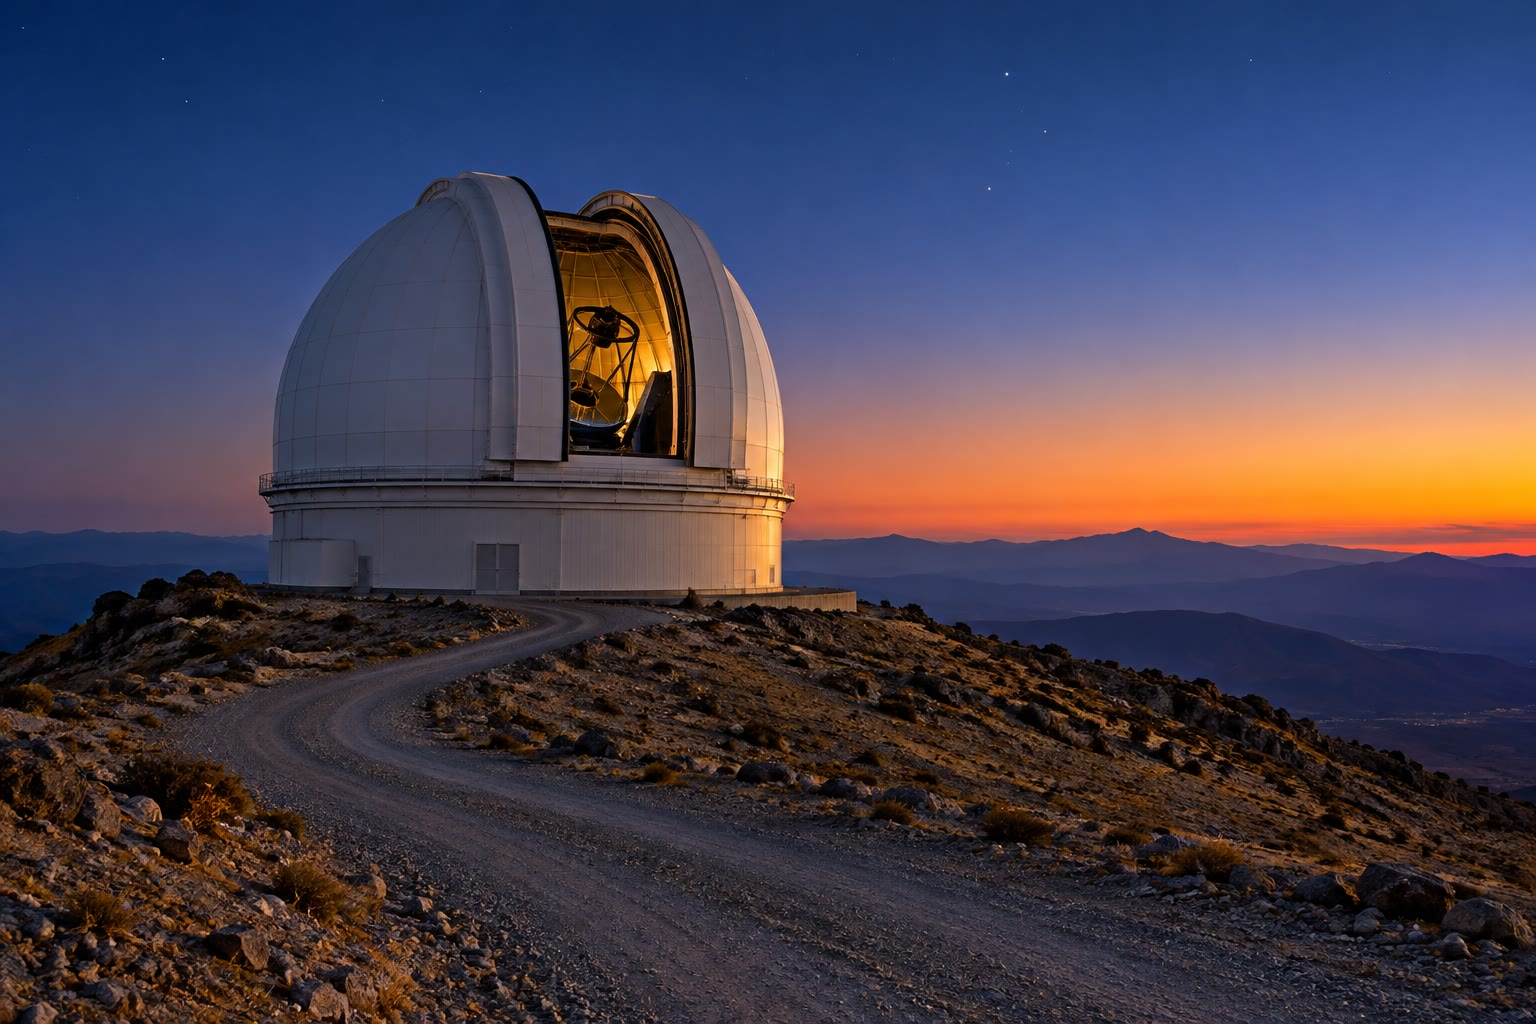
\includegraphics[width=0.55\linewidth]{images/book3/ai/b1-observatory-dusk.jpg}
\end{center}
\end{inthefield}

\section{Flujos y magnitudes}\label{sec:b1:observing-the-sky:magnitudes}

\begin{definition}[Flujo, luminosidad]\label{def:b1:observing-the-sky:flux}
El \emph{flujo}\index{flujo (de una fuente)} $F$ que recibimos de una fuente es la
potencia de su radiación que atraviesa una unidad de área colocada perpendicularmente a
su dirección, en vatios por metro cuadrado; restringido a una banda de longitudes de
onda, es el flujo en esa banda. La \emph{luminosidad}\index{luminosidad} $L$ de la fuente
es la potencia total que radia, en vatios.
\end{definition}

\begin{proposition}[Ley de la inversa del cuadrado]\label{prop:b1:observing-the-sky:inverse-square}
Una fuente de \omterm{def:b1:observing-the-sky:flux}{luminosidad} $L$ que radia por igual en todas las direcciones, vista a una
distancia $d$ a través del espacio vacío, da el \omterm{def:b1:observing-the-sky:flux}{flujo}
\[
  F = \frac{L}{4\pi d^2} .
\]
\end{proposition}

\begin{proof}
En un régimen estacionario, sin absorción, la potencia que atraviesa cualquier esfera
centrada en la fuente es la misma, $L$, por conservación de la energía. Por simetría se
reparte uniformemente sobre el área de la esfera, $4\pi d^2$.
\end{proof}

\begin{example}
El \omterm{def:b1:observing-the-sky:flux}{flujo} de la \omterm{def:b1:observing-the-sky:flux}{luminosidad} del Sol, de \qty{3.828e26}{W}, a una unidad astronómica,
\qty{1.496e11}{m}, es $\num{3.828e26}/(4\pi\times
(\num{1.496e11})^2) = \qty{1361}{W.m^{-2}}$: la irradiancia solar que recibe la Tierra en
el alto de su atmósfera.
% ledger: sun:L, const:au, earth:TSI
\end{example}

Los \omterm{def:b1:observing-the-sky:flux}{flujos} abarcan un rango enorme, y los astrónomos los comparan en una escala
logarítmica heredada de las clases en que se ordenaban las estrellas visibles a simple
vista: las más brillantes, de primera magnitud, y las más débiles, de sexta.

\begin{definition}[Magnitud aparente, banda fotométrica]\label{def:b1:observing-the-sky:magnitude}
Una \emph{banda fotométrica}\index{banda fotométrica} es una franja de longitudes de onda
seleccionada por un filtro estándar y designada por una letra: U (ultravioleta), B (azul),
V (visual), R (rojo), I (infrarrojo cercano), y J, H, K en las ventanas infrarrojas. La
\emph{magnitud aparente}\index{magnitud aparente} $m$ de una fuente en una banda se define
a partir de su \omterm{def:b1:observing-the-sky:flux}{flujo} $F$ en esa banda mediante
\[
  m_1 - m_2 = -2.5\log_{10}\frac{F_1}{F_2} ,
\]
con el punto cero fijado por estrellas patrón, cercano a la magnitud de la estrella Vega
en cada banda. Una diferencia de 5 magnitudes equivale a un factor de exactamente 100 en el
\omterm{def:b1:observing-the-sky:flux}{flujo}; una magnitud equivale a un factor $100^{1/5} = 2.512$. Las fuentes más brillantes
tienen magnitudes más pequeñas, y posiblemente negativas.
\end{definition}

Las longitudes de onda centrales de los filtros estándar U, B, V, R e I son
\qty{358.5}{nm}, \qty{437.1}{nm}, \qty{547.8}{nm}, \qty{650.4}{nm} y
\qty{802.0}{nm}.
% ledger: baldry:bessell-pivot
En la banda V, el Sol tiene una \omterm{def:b1:observing-the-sky:magnitude}{magnitud aparente} de $-26.74$, Sirio, la estrella más
brillante del cielo nocturno, $-1.46$, y Vega $0.03$. El Sol es, pues,
$10^{0.4\times(26.74 - 1.46)} = \num{1.29e10}$ veces más brillante que Sirio en nuestro
cielo; eso no dice todavía cuál de las dos brilla más de verdad, para lo cual hacen falta
las distancias.
% ledger: nasa:sun-V, simbad:sirius, simbad:vega

\subsection*{Paralaje y parsec}

A medida que la Tierra gira alrededor del Sol, una estrella cercana parece desplazarse
frente a las estrellas de fondo, mucho más lejanas, describiendo en un año una pequeña
elipse. Ese movimiento aparente es la medida más directa de las distancias estelares: usa
la órbita terrestre como base de triangulación de un agrimensor.

\begin{definition}[Paralaje anual, parsec]\label{def:b1:observing-the-sky:parallax}
La \emph{paralaje anual}\index{paralaje anual} $p$ de una estrella es el ángulo que
subtiende en la estrella el radio de la órbita terrestre, una unidad astronómica, visto
perpendicularmente a la visual; es el semieje mayor de
la elipse anual que parece describir la estrella. El \emph{parsec}\index{parsec}
(\unit{\parsec}) es la distancia a la que una unidad astronómica subtiende un segundo
de arco:
\[
  \qty{1}{\parsec} = \frac{\qty{1}{\au}}{\tan\ang{;;1}} = \qty{206265}{\au}
  = \qty{3.0857e16}{m} = \qty{3.2616}{\lightyear} .
\]
\end{definition}

Como $p$ es muy pequeño, $\tan p \approx p$ en radianes, y la distancia se obtiene de
inmediato:
\[
  d = \frac{\qty{1}{\au}}{\tan p} \quad\Longrightarrow\quad
  \frac{d}{\unit{\parsec}} = \frac{1}{p/\text{arcsec}} .
\]
La paralaje de Sirio es \ang{;;0.37921}, así que se encuentra a $1/0.37921 =
\qty{2.637}{\parsec}$, es decir, \qty{8.60}{\lightyear}. Incluso las estrellas más
cercanas tienen paralajes inferiores a un segundo de arco, más pequeñas que el \omterm{def:b1:observing-the-sky:seeing}{seeing}: la
paralaje se halla a partir del desplazamiento del centro de la imagen de la estrella, que
muchos fotones localizan con una precisión mucho mayor que la anchura de la imagen. Una
misión espacial descrita al final de este capítulo ha medido de este modo las posiciones
de casi dos mil millones de objetos.
% ledger: simbad:sirius, const:au, esa:gaia

\begin{omfigure}
\begin{tikzpicture}[font=\small]
\draw[black!50] (0,0) ellipse (2.0cm and 0.55cm);
\fill[orange!80!black] (0,0) circle (3pt) node[below=3pt] {Sol};
\fill[blue!70!black] (-2.0,0) circle (2pt) node[left, align=right] {Tierra, seis\\ meses después};
\fill[blue!70!black] (2.0,0) circle (2pt) node[right] {Tierra};
\fill (0,4.4) circle (1.6pt) node[above] {estrella};
\draw[omDef, thick] (0,0) -- node[right, pos=0.55] {$d$} (0,4.4);
\draw[omThm] (2.0,0) -- (0,4.4);
\draw[omThm, dashed] (-2.0,0) -- (0,4.4);
\draw[thick] (0,0) -- node[above] {\qty{1}{\au}} (2.0,0);
\draw[omThm] (0,3.75) arc[start angle=-90, end angle=-65.6, radius=0.65cm];
\node[omThm] at (0.17,3.38) {$p$};
\end{tikzpicture}

{\small \omterm{def:b1:observing-the-sky:parallax}{Paralaje anual} (no a escala): vista desde la estrella, el radio de la órbita
terrestre subtiende el ángulo $p$. Con seis meses de diferencia, la dirección de la
estrella cambia en $2p$. El ángulo real de la estrella más cercana es inferior a un
segundo de arco.}
\end{omfigure}

\begin{definition}[Magnitud absoluta, módulo de distancia]\label{def:b1:observing-the-sky:absolute}
La \emph{magnitud absoluta}\index{magnitud absoluta} $M$ de una estrella en una banda es
la \omterm{def:b1:observing-the-sky:magnitude}{magnitud aparente} que tendría a la distancia de \qty{10}{\parsec}, vista a través del
espacio vacío. La diferencia $m - M$ es su
\emph{módulo de distancia}\index{módulo de distancia}.
\end{definition}

\begin{proposition}[El módulo de distancia]\label{prop:b1:observing-the-sky:modulus}
Para una estrella a la distancia $d$ vista a través del espacio vacío,
\[
  m - M = 5\log_{10}\frac{d}{\qty{10}{\parsec}} .
\]
Si la luz se atenúa en su camino por $A$ magnitudes de extinción,
$m - M = 5\log_{10}(d/\qty{10}{\parsec}) + A$. En una banda, el cociente de las
\omterm{def:b1:observing-the-sky:flux}{luminosidades} de dos estrellas es $L_1/L_2 = 10^{0.4(M_2 - M_1)}$.
\end{proposition}

\begin{proof}
Por la ley de la inversa del cuadrado, el \omterm{def:b1:observing-the-sky:flux}{flujo} a $d$ y el \omterm{def:b1:observing-the-sky:flux}{flujo} a \qty{10}{\parsec}
están en la razón $F(d)/F(\qty{10}{\parsec}) = (\qty{10}{\parsec}/d)^2$. La definición de
las magnitudes da $m - M = -2.5\log_{10}(\qty{10}{\parsec}/d)^2
= 5\log_{10}(d/\qty{10}{\parsec})$. La extinción multiplica el \omterm{def:b1:observing-the-sky:flux}{flujo} por
$10^{-0.4A}$, lo que suma $A$ a $m$. A la distancia común de
\qty{10}{\parsec}, los \omterm{def:b1:observing-the-sky:flux}{flujos} están en la razón de las \omterm{def:b1:observing-the-sky:flux}{luminosidades}, y
$M_1 - M_2 = -2.5\log_{10}(L_1/L_2)$.
\end{proof}

El Sol tiene una \omterm{def:b1:observing-the-sky:absolute}{magnitud absoluta} $M_\odot = 4.83$ y una \omterm{def:b1:observing-the-sky:flux}{luminosidad} de
\qty{3.828e26}{W}. Comparando la \omterm{def:b1:observing-the-sky:absolute}{magnitud absoluta} de una estrella en V con la del Sol
se obtiene su \omterm{def:b1:observing-the-sky:flux}{luminosidad} en V en unidades solares,
$L/L_\odot = 10^{0.4(4.83 - M)}$ --- una \omterm{def:b1:observing-the-sky:flux}{luminosidad} en la \emph{banda V}, ya que una
estrella mucho más caliente o más fría que el Sol emite otra parte de su potencia fuera
de la banda V.
% ledger: sun:Mabs, sun:L

\subsection*{Color}

\begin{definition}[Índice de color]\label{def:b1:observing-the-sky:colour-index}
El \emph{índice de color}\index{índice de color} de una estrella es la diferencia de sus
magnitudes en dos bandas, primero la más azul; el más usado es $B - V$. Un $B - V$ pequeño
o negativo indica una estrella azul, y uno grande, una estrella roja.
\end{definition}

El \omterm{def:b1:observing-the-sky:colour-index}{índice de color} no depende de la distancia, pues la ley de la inversa del cuadrado
atenúa ambas bandas por igual; mide la forma del espectro y, con ella, la temperatura de
la superficie de la estrella. Una estrella radia más o menos como un cuerpo negro cuyo
espectro tiene el máximo en $\lambda_\mathrm{max} = b/T$ (ley de Wien, con
$b = \qty{2.898e-3}{m.K}$, que se toma del libro de física de segundo año).
La figura siguiente dibuja tres espectros de cuerpo negro: un cuerpo frío a
\qty{3500}{K} tiene el máximo en el infrarrojo cercano y da más \omterm{def:b1:observing-the-sky:flux}{flujo} en V que en B; la
temperatura efectiva del Sol, \qty{5772}{K}, sitúa su máximo en \qty{502}{nm}, entre B y
V; un cuerpo a \qty{10000}{K} tiene el máximo en el ultravioleta y es más brillante en B
que en V. El cociente entre las radiancias en B y en V crece de forma constante con la
temperatura, de \num{0.46} a \num{0.97} y \num{1.53} en las tres curvas, y por eso
$B - V$ disminuye al aumentar $T$.
% ledger: const:b, nasa:sun-Teff, baldry:bessell-pivot

\begin{omfigure}
\begin{tikzpicture}
\begin{axis}[omrecord, width=0.9\linewidth, height=5.8cm, xmin=200, xmax=1500,
  ymin=0, ymax=1.17, xtick={200,400,...,1400}, ytick={0,0.5,1},
  xlabel={longitud de onda (nm)},
  ylabel={$B_\lambda$ / máximo}, tick label style={font=\scriptsize},
  label style={font=\small}, legend style={font=\scriptsize, at={(0.5,1.03)},
  anchor=south, draw=none, fill=none}, legend columns=3]
\addplot[red!75!black, line width=1.1pt] table[x=lam_nm, y=t3500] {figdata/out/bachelor-1-blackbody_bands-curves.dat};
\addplot[orange!90!black, line width=1.1pt] table[x=lam_nm, y=t5772] {figdata/out/bachelor-1-blackbody_bands-curves.dat};
\addplot[omDef, line width=1.1pt] table[x=lam_nm, y=t10000] {figdata/out/bachelor-1-blackbody_bands-curves.dat};
\legend{\qty{3500}{K}, \qty{5772}{K} (el Sol), \qty{10000}{K}}
\draw[black!45, densely dashed] (axis cs:358.5,0) -- (axis cs:358.5,1.06);
\node[font=\scriptsize, above, inner sep=1pt] at (axis cs:358.5,1.06) {U};
\draw[black!45, densely dashed] (axis cs:437.1,0) -- (axis cs:437.1,1.06);
\node[font=\scriptsize, above, inner sep=1pt] at (axis cs:437.1,1.06) {B};
\draw[black!45, densely dashed] (axis cs:547.8,0) -- (axis cs:547.8,1.06);
\node[font=\scriptsize, above, inner sep=1pt] at (axis cs:547.8,1.06) {V};
\draw[black!45, densely dashed] (axis cs:650.4,0) -- (axis cs:650.4,1.06);
\node[font=\scriptsize, above, inner sep=1pt] at (axis cs:650.4,1.06) {R};
\draw[black!45, densely dashed] (axis cs:802.0,0) -- (axis cs:802.0,1.06);
\node[font=\scriptsize, above, inner sep=1pt] at (axis cs:802.0,1.06) {I};
\end{axis}
\end{tikzpicture}

{\small Espectros de cuerpo negro a tres temperaturas, dividido cada uno por su propio
máximo, con las longitudes de onda centrales de los filtros U, B, V, R e I (trazos).
El máximo se desplaza a longitudes de onda más cortas al aumentar la temperatura (ley
de Wien): \qty{828}{nm}, \qty{502}{nm} y \qty{290}{nm}.}
% ledger: const:h, const:c, const:kB, const:b, nasa:sun-Teff, baldry:bessell-pivot
\end{omfigure}

Cuatro estrellas brillantes muestran la gama de colores:
\begin{center}
\small
\begin{tabular}{lcccc}
\hline
estrella & $V$ & $B$ & $B - V$ & paralaje (\unit{mas}) \\
\hline
Rigel & 0.13 & 0.10 & $-0.03$ & 3.78 \\
Altair & 0.76 & 0.98 & 0.22 & 194.95 \\
Polaris & 2.02 & 2.62 & 0.60 & 7.54 \\
Betelgeuse & 0.42 & 2.27 & 1.85 & 6.55 \\
\hline
\end{tabular}
\end{center}
% ledger: simbad:rigel, simbad:altair, simbad:polaris, simbad:betelgeuse
Rigel es blanca azulada y Betelgeuse, en la misma constelación, naranja rojiza: una
diferencia de color visible a simple vista. Sus tipos espectrales, B8 y M1--M2, dicen lo
mismo en el lenguaje de los espectros, tema del libro 5, tercer año.

\section{Espectrógrafos}

La fotometría mide la luz en unas pocas bandas anchas; un espectrógrafo la extiende en un
espectro. La luz del foco del telescopio atraviesa una rendija estrecha, se hace paralela
con un colimador, se dispersa en una red de difracción (o en un prisma) y una cámara la
enfoca sobre el detector, donde cada longitud de onda cae en una columna distinta de
píxeles (véase la figura siguiente). Una red con $N$ líneas iluminadas, usada en el orden
$k$, separa dos longitudes de onda separadas $\Delta\lambda$ cuando $\lambda/\Delta\lambda \le kN$:
es su poder resolutor (recordado del libro de física de segundo año).

\begin{omfigure}
\begin{tikzpicture}[font=\scriptsize, >=Stealth]
\draw[thick, fill=omSea!25] (0.15,0) ellipse (0.13 and 0.9);
\node[below] at (0.15,-0.95) {objetivo};
\draw[omDef] (-1.3,0.75) -- (0.15,0.75) -- (2.4,0);
\draw[omDef] (-1.3,-0.75) -- (0.15,-0.75) -- (2.4,0);
\draw[omDef, ->] (-1.3,0) -- (-0.2,0);
\node[above] at (-0.8,0.75) {luz estelar};
\draw[very thick] (2.4,-0.35) -- (2.4,-0.06); \draw[very thick] (2.4,0.06) -- (2.4,0.35);
\node[above] at (2.4,0.38) {rendija};
\draw[omDef] (2.4,0) -- (3.6,0.55); \draw[omDef] (2.4,0) -- (3.6,-0.55);
\draw[thick, fill=omSea!25] (3.6,0) ellipse (0.1 and 0.72); \node[below] at (3.6,-0.74) {colimador};
\draw[omDef] (3.6,0.55) -- (4.9,0.55); \draw[omDef] (3.6,-0.55) -- (4.9,-0.55);
\draw[thick, pattern=north east lines] (4.85,-0.8) rectangle (5.0,0.8);
\node[below] at (4.92,-0.82) {red de difracción};
\draw[blue!70!black] (5.0,0.3) -- (6.4,0.95); \draw[red!70!black] (5.0,0.3) -- (6.4,-0.15);
\draw[blue!70!black] (5.0,-0.3) -- (6.4,0.35); \draw[red!70!black] (5.0,-0.3) -- (6.4,-0.75);
\draw[thick, fill=omSea!25] (6.4,0.1) ellipse (0.1 and 1.08); \node[below] at (6.4,-1.0) {cámara};
\draw[blue!70!black] (6.4,0.95) -- (7.6,0.55); \draw[blue!70!black] (6.4,0.35) -- (7.6,0.55);
\draw[red!70!black] (6.4,-0.15) -- (7.6,-0.45); \draw[red!70!black] (6.4,-0.75) -- (7.6,-0.45);
\fill[black!70] (7.6,-0.8) rectangle (7.75,0.9);
\node[right, align=left] at (7.8,0.05) {detector:\\ una longitud de onda\\ por columna};
\end{tikzpicture}

{\small El camino de la luz por un telescopio y un espectrógrafo de red (esquema, con el
objetivo del telescopio y la óptica dibujados como lentes, y dos longitudes de onda): la
rendija aísla la imagen de la estrella, el colimador vuelve paralelo el haz, la red lo
dispersa y la cámara enfoca cada longitud de onda sobre su propio lugar del detector.}
\end{omfigure}

Un espectro lleva tres clases de información. Sus \emph{líneas}, oscuras donde los átomos y
iones de la atmósfera de la estrella absorben, brillantes donde un gas caliente y tenue
emite, identifican los elementos químicos presentes. La forma de su continuo, y las
intensidades relativas de las líneas formadas a distintas temperaturas, dan la temperatura
del gas. Y el desplazamiento Doppler de las líneas da la velocidad a lo largo de la visual:
una línea de longitud de onda en reposo $\lambda$ se desplaza en $\Delta\lambda = \lambda v_r/c$
para una velocidad radial $v_r$ mucho menor que $c$. Medir $v_r$ con una precisión de
\qty{1}{km.s^{-1}} exige un poder resolutor del orden de $c/v_r = \num{300000}$, o un poder
resolutor moderado y muchas líneas medidas en conjunto. Cómo los espectros revelan la
estructura, la composición y los movimientos de estrellas y galaxias es el tema del libro 5,
tercer año.

\section{Observación desde el espacio}

Por encima de la atmósfera no hay ventanas cerradas, ni extinción, ni \omterm{def:b1:observing-the-sky:seeing}{seeing}, y en el
infrarrojo no hay resplandor del aire caliente. Los telescopios espaciales pagan esto con
coste, con la masa y el tamaño limitados que puede lanzar un cohete y, en la mayoría de
los casos, con la imposibilidad de repararlos. Se usan donde el suelo no puede competir:
para los rayos gamma, los rayos X y la luz ultravioleta, que nunca llegan al suelo; para
el infrarrojo más allá de las ventanas estrechas; para imágenes en el límite de difracción
sobre un campo amplio; y para medidas, como las paralajes de muchísimas estrellas, que
necesitan un instrumento estable fuera del aire turbulento.

\begin{dated}{2026}
% ledger: nasa:hubble-mirror, nasa:jwst-mirror, nasa:jwst-orbit, nasa:jwst-launch, nasa:jwst-range, esa:gaia
Tres observatorios espaciales muestran la gama. El Telescopio Espacial Hubble,
lanzado en 1990, tiene un espejo primario de \qty{2.4}{m} de diámetro. El Telescopio
Espacial James Webb, lanzado el 25 de diciembre de 2021, tiene un espejo primario de
\qty{6.5}{m} formado por 18 segmentos hexagonales, con un área colectora de
\qty{25}{m^2}; trabaja desde \qty{0.6}{\micro\metre} hasta \qty{28.5}{\micro\metre} y
orbita el Sol cerca del segundo punto de Lagrange, L2, a \num{1.5} millones de kilómetros
de la Tierra, en el lado opuesto al Sol. Gaia, lanzado el 19 de diciembre de 2013 a la
misma región, usó dos telescopios sobre un plano focal común de CCD para cartografiar las
posiciones y los movimientos de casi dos mil millones de objetos en tres dimensiones; sus
observaciones han terminado y sus catálogos se están publicando.
\end{dated}

\begin{omfigure}
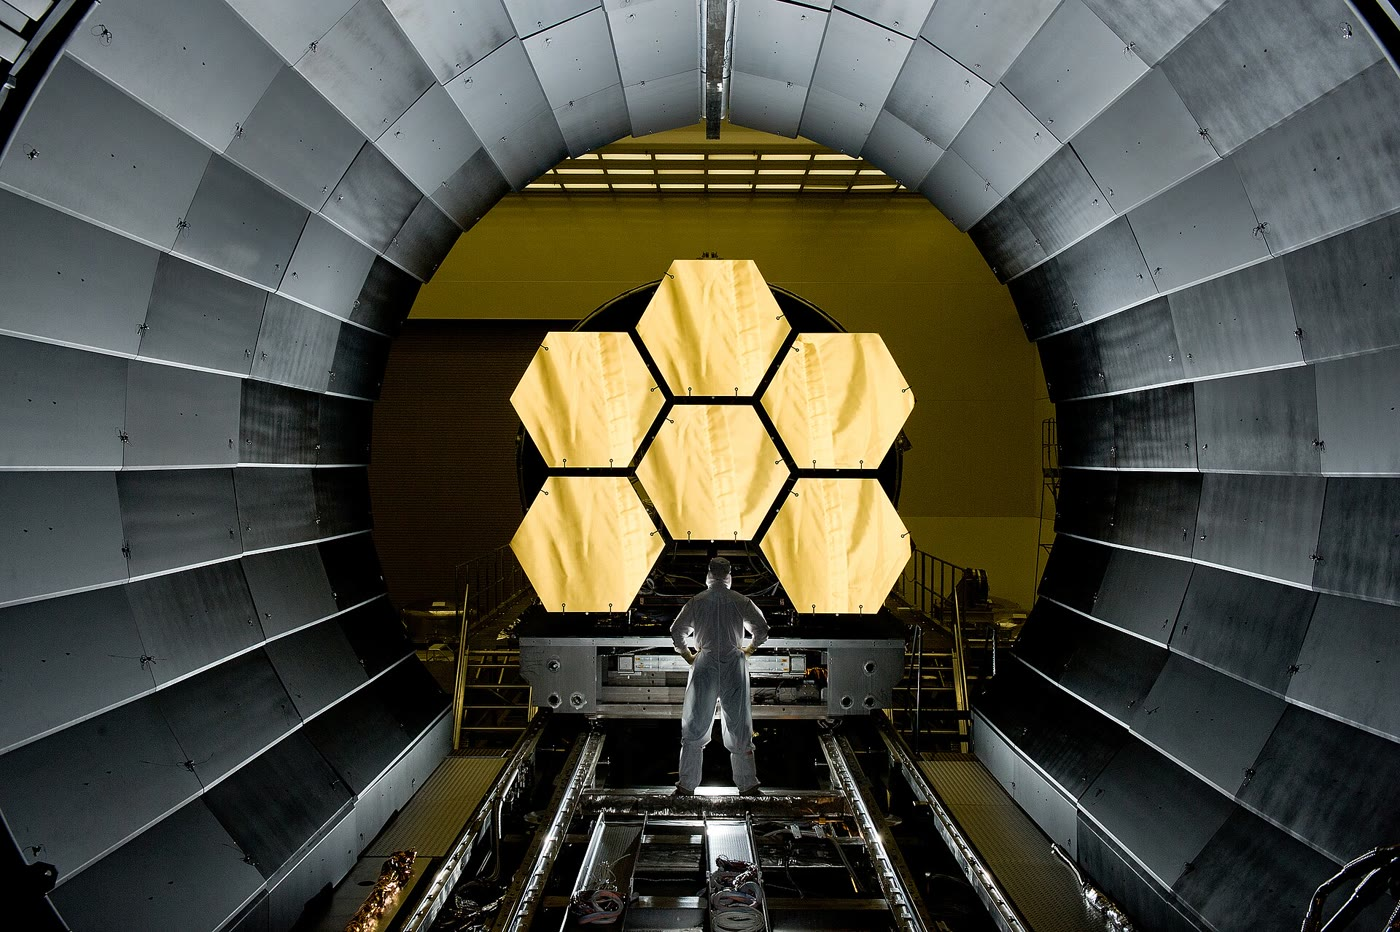
\includegraphics[width=0.78\linewidth]{images/book3/b1-jwst-mirror-segments.jpg}

{\small Seis de los 18 segmentos hexagonales del espejo primario del Telescopio Espacial
James Webb, preparados para las pruebas en frío en 2011; desplegados en el espacio, los 18
forman un espejo de \qty{6.5}{m} de ancho. Fotografía NASA/MSFC/David Higginbotham,
dominio público.}
% ledger: commons:jwst-mirror, nasa:jwst-mirror
\end{omfigure}

\section{Ejercicios}

\begin{exercise}[$\star$]\label{exo:b1:observing-the-sky:1}
Calcúlese el cociente de los \omterm{def:b1:observing-the-sky:flux}{flujos} de dos estrellas de magnitudes 1.0 y 6.0. ¿Y el de
Rigel ($V = 0.13$) y Polaris ($V = 2.02$)? ¿Cuál brilla más en el cielo?
\end{exercise}

\begin{exercise}[$\star$]\label{exo:b1:observing-the-sky:2}
La paralaje de Altair es \ang{;;0.19495}. Dése su distancia en \omterm{def:b1:observing-the-sky:parallax}{parsecs}, en unidades
astronómicas y en años luz.
\end{exercise}

\begin{exercise}[$\star$]\label{exo:b1:observing-the-sky:3}
Calcúlese el límite de difracción de un telescopio espacial de \qty{2.4}{m} a
\qty{550}{nm}, en segundos de arco, y compárese con un \omterm{def:b1:observing-the-sky:seeing}{seeing} de \ang{;;0.40}. Repítase
para un telescopio de \qty{6.5}{m} a \qty{2.0}{\micro\metre}.
\end{exercise}

\begin{exercise}[$\star$]\label{exo:b1:observing-the-sky:4}
A partir de la tabla de las cuatro estrellas brillantes, ordénense Rigel, Altair, Polaris
y Betelgeuse de la superficie más caliente a la más fría. ¿Por qué puede compararse el
\omterm{def:b1:observing-the-sky:colour-index}{índice de color} entre estrellas a distancias muy diferentes?
\end{exercise}

\begin{exercise}[$\star\star$]\label{exo:b1:observing-the-sky:5}
Una estrella se mide con magnitud 6.412 a la distancia cenital \ang{30} y con 6.590 a
\ang{60} la misma noche. Suponiendo una atmósfera plano-paralela, calcúlense las dos \omterm{def:b1:observing-the-sky:extinction}{masas
de aire}, el coeficiente de extinción y la magnitud de la estrella por encima de la atmósfera.
\end{exercise}

\begin{exercise}[$\star\star$]\label{exo:b1:observing-the-sky:6}
Una estrella da 400 fotoelectrones en una exposición de \qty{10}{s}, y domina el ruido de
fotones de la propia estrella. ¿Cuál es la \omterm{def:b1:observing-the-sky:detector}{relación señal-ruido}? ¿Cuánto hay que exponer
para alcanzar una \omterm{def:b1:observing-the-sky:detector}{relación señal-ruido} de 100? ¿Y para medir la magnitud con un error de
\num{0.01}?
\end{exercise}

\begin{exercise}[$\star\star$]\label{exo:b1:observing-the-sky:7}
Rigel tiene $V = 0.13$ y una paralaje de \ang{;;0.00378}. Despreciando la extinción entre
ella y nosotros, calcúlese su distancia, su \omterm{def:b1:observing-the-sky:absolute}{magnitud absoluta} y su \omterm{def:b1:observing-the-sky:flux}{luminosidad} en V en
unidades solares ($M_\odot = 4.83$).
\end{exercise}

\begin{exercise}[$\star\star$]\label{exo:b1:observing-the-sky:8}
Compárense las áreas colectoras de un espejo circular de \qty{2.4}{m} (sin tener en cuenta
su obstrucción central) y del telescopio Webb (\qty{25}{m^2}). ¿Cuánto más corta es la
exposición en la que el telescopio Webb recoge el mismo número de fotones? ¿Qué fracción de
un disco completo de \qty{6.5}{m} de diámetro representa su área colectora, y por qué es
menor que uno?
\end{exercise}

\begin{exercise}[$\star\star$]\label{exo:b1:observing-the-sky:9}
(a) A partir de la \omterm{def:b1:observing-the-sky:flux}{luminosidad} del Sol, \qty{3.828e26}{W}, calcúlese su \omterm{def:b1:observing-the-sky:flux}{flujo} a
\qty{10}{\parsec}. (b) Las \omterm{def:b1:observing-the-sky:magnitude}{magnitudes aparente} y absoluta del Sol son $-26.74$ y $4.83$.
Úsese el \omterm{def:b1:observing-the-sky:absolute}{módulo de distancia} para recuperar la distancia Sol--Tierra, en unidades
astronómicas.
\end{exercise}

\begin{exercise}[$\star\star\star$]\label{exo:b1:observing-the-sky:10}
Demuéstrese a partir de \cref{prop:b1:observing-the-sky:bouguer} que $k =
2.5\log_{10}e\;\tau_0$. Para la noche de la recta de extinción ($k =
\num{0.160}$), calcúlese la profundidad óptica en el \omterm{def:b1:spherical-astronomy:celestial-sphere}{cenit} $\tau_0$ y la fracción de la luz
que llega al telescopio en el \omterm{def:b1:spherical-astronomy:celestial-sphere}{cenit} y a $X = 2.31$. ¿Qué predice una atmósfera
plano-paralela para la \omterm{def:b1:observing-the-sky:extinction}{masa de aire} a una distancia cenital de \ang{85}, y por qué no debe
confiarse en ese valor?
\end{exercise}

\begin{exercise}[$\star\star\star$]\label{exo:b1:observing-the-sky:11}
Una galaxia débil da $R = 50$ fotoelectrones por segundo en un telescopio, y el cielo en el
área de su imagen da $B = \num{2000}$ por segundo cuando el \omterm{def:b1:observing-the-sky:seeing}{seeing} es \ang{;;0.80}. El ruido
de lectura es despreciable. (a) ¿Cuánto hay que exponer para una \omterm{def:b1:observing-the-sky:detector}{relación señal-ruido} de 10?
(b) El cielo en la imagen crece con el área del disco de \omterm{def:b1:observing-the-sky:seeing}{seeing}. Repítase para un \omterm{def:b1:observing-the-sky:seeing}{seeing} de
\ang{;;0.40}. (c) Demuéstrese que, para una fuente mucho más débil que el cielo, el tiempo de
exposición necesario para una \omterm{def:b1:observing-the-sky:detector}{relación señal-ruido} dada varía como $\theta^2/D^2$, donde
$\theta$ es el \omterm{def:b1:observing-the-sky:seeing}{seeing} y $D$ el diámetro del telescopio.
\end{exercise}

\begin{exercise}[$\star\star\star$]\label{exo:b1:observing-the-sky:12}
Una red de 1200 líneas por milímetro se ilumina sobre \qty{100}{mm} y se usa en el primer
orden. (a) ¿Cuál es su poder resolutor, y cuál es la menor diferencia de longitud de onda
separable a \qty{550}{nm}? (b) ¿A qué velocidad radial corresponde esa diferencia? (c) La
Tierra se mueve alrededor del Sol a \qty{29.78}{km.s^{-1}}. ¿En cuánto puede desplazar ese
movimiento una línea a \qty{550}{nm}, y cuántos elementos de resolución son? ¿Qué debe
hacer, por tanto, un observador que mide la velocidad de una estrella?
% ledger: earth:vorb
\end{exercise}

\section{Problema: pesar la luz de Sirio}

\begin{problem}[{Problema de fin de semana --- a qué distancia está Sirio, cuánto brilla y
cuántos fotones envía, y cuántos soles supera en brillo}]
\label{pb:b1:observing-the-sky:1}
% ledger: simbad:sirius, simbad:vega, simbad:sirius-b, nasa:sun-V, sun:Mabs, const:au
% numbers computed in the scratch calculator calc/ch02.py from the rounded data
Sirio, la estrella más brillante del cielo nocturno, tiene una compañera débil, la enana
blanca Sirio~B. Utilícense los datos:
\begin{center}
\small
\begin{tabular}{lcc}
\hline
objeto & $V$ & paralaje \\
\hline
Sirio & $-1.46$ & \ang{;;0.37921} \\
Sirio B & $8.44$ & --- \\
Vega & $0.03$ & \ang{;;0.13023} \\
el Sol & $-26.74$ & --- \\
\hline
\end{tabular}
\end{center}
con $M_\odot = 4.83$ en V, $\qty{1}{\parsec} = \qty{206265}{\au} =
\qty{3.0857e16}{m} = \qty{3.2616}{\lightyear}$, y un coeficiente de extinción
$k = 0.15$ por \omterm{def:b1:observing-the-sky:extinction}{masa de aire} en el observatorio.

\medskip
\noindent\textbf{Parte I --- ¿A qué distancia está Sirio?}
\begin{enumerate}
  \item Calcúlese la distancia de Sirio en \omterm{def:b1:observing-the-sky:parallax}{parsecs}.
  \item Exprésese en unidades astronómicas y en metros.
  \item Exprésese en años luz. ¿Cuánto tiempo hace que la luz que vemos esta noche
        salió de Sirio?
  \item En el transcurso de un año, ¿qué ángulo total recorre la dirección de Sirio de un
        lado a otro? Compárese con un \omterm{def:b1:observing-the-sky:seeing}{seeing} de \ang{;;0.40}. ¿Por qué puede medirse aún
        el balanceo hasta una pequeña fracción del \omterm{def:b1:observing-the-sky:seeing}{seeing}?
  \item Si la paralaje estuviera equivocada en \ang{;;0.001}, ¿en qué fracción sería
        errónea la distancia, y en cuántos años luz?
\end{enumerate}

\medskip
\noindent\textbf{Parte II --- ¿Cuánto brilla?}
\begin{enumerate}[resume]
  \item Calcúlese el cociente de los \omterm{def:b1:observing-the-sky:flux}{flujos} de Sirio y de Vega en V.
  \item Calcúlese el cociente de los \omterm{def:b1:observing-the-sky:flux}{flujos} del Sol y de Sirio.
  \item Calcúlese el cociente de los \omterm{def:b1:observing-the-sky:flux}{flujos} de Sirio y de Sirio~B.
  \item Desde el Observatorio de Paranal, Sirio cruza el meridiano a una altura de
        \ang{82.09} (\cref{ch:b1:spherical-astronomy}). Calcúlense la \omterm{def:b1:observing-the-sky:extinction}{masa de aire}, la
        extinción y la magnitud medida en ese momento.
  \item Repítase a una altura de \ang{30}. ¿Qué fracción de la luz se pierde en el camino?
  \item ¿Por qué la fórmula $X = \sec z$ induciría a error a un observador que mide Sirio
        justo después de salir?
\end{enumerate}

\medskip
\noindent\textbf{Parte III --- Contar fotones.}
Una cámara en un telescopio de \qty{1}{m} registra $\num{3.0e4}$ fotoelectrones por
segundo de una estrella de magnitud $V = 10.0$, una vez corregida la extinción. Cada píxel
guarda como máximo $\num{1.0e5}$ electrones (su pozo lleno).
\begin{enumerate}[resume]
  \item ¿Cuántos fotoelectrones por segundo registra la cámara de Sirio~B?
  \item ¿Cuánto debe durar una exposición para que Sirio~B tenga una \omterm{def:b1:observing-the-sky:detector}{relación
        señal-ruido} de 1000, con ruido de fotones solo de la estrella? ¿Cuál es entonces el
        error en su magnitud?
  \item ¿Cuántos fotoelectrones por segundo registra la cámara de Sirio?
  \item Si el \qty{20}{\percent} de la luz de Sirio cae en su píxel más brillante, ¿cuánto
        tarda en llenarse ese píxel?
  \item En la imagen, las alas débiles de la imagen de Sirio depositan, en el lugar de
        Sirio~B, $10^{-4}$ de la luz de Sirio por píxel, y el píxel más brillante de Sirio~B
        recoge el \qty{20}{\percent} de su propia luz. Compárense las dos tasas en ese píxel.
  \item ¿Cuál es la exposición más larga que no satura ese píxel? Calcúlese la \omterm{def:b1:observing-the-sky:detector}{relación
        señal-ruido} de Sirio~B en ese píxel en una exposición de \qty{0.5}{s}, contando el
        ruido de fotones de ambas fuentes. ¿Es detectable Sirio~B, y qué lo hace difícil?
\end{enumerate}

\medskip
\noindent\textbf{Parte IV --- ¿Cuántos soles?}
\begin{enumerate}[resume]
  \item Calcúlese el \omterm{def:b1:observing-the-sky:absolute}{módulo de distancia} de Sirio.
  \item Dedúzcase la \omterm{def:b1:observing-the-sky:absolute}{magnitud absoluta} de Sirio en V, con dos decimales.
  \item Calcúlese la distancia y la \omterm{def:b1:observing-the-sky:absolute}{magnitud absoluta} de Vega.
  \item ¿Cuál de Sirio y de Vega es intrínsecamente más luminosa en V, y en qué factor?
  \item ¿Cuál sería la \omterm{def:b1:observing-the-sky:magnitude}{magnitud aparente} del Sol visto desde la distancia de Sirio? Tomando
        6.0 como la magnitud más débil visible a simple vista en una noche oscura, ¿sería
        visible?
  \item ¿Hasta qué distancia seguiría siendo visible Sirio a simple vista?
  \item Calcúlese la \omterm{def:b1:observing-the-sky:flux}{luminosidad} de Sirio en V en unidades solares: ¿cuántos soles supera
        Sirio en brillo?
\end{enumerate}
\end{problem}
